\documentclass[conference]{IEEEtran}
\IEEEoverridecommandlockouts

\usepackage{cite}
\usepackage{amsmath,amssymb,amsfonts}
\usepackage{graphicx}
\usepackage{textcomp}
\usepackage{xcolor}
\usepackage{float}
\usepackage{hyperref}
\usepackage{listings}

\def\BibTeX{{\rm B\kern-.05em{\sc i\kern-.025em b}\kern-.08em
    T\kern-.1667em\lower.7ex\hbox{E}\kern-.125emX}}
\begin{document} 


\title{Noise Analysis}

\author{\IEEEauthorblockN{Emmanuel Jesus R. Estallo}
\IEEEauthorblockA{\textit{Electrical and Electronics Engineering Institute} \\
\textit{University of the Philippines - Diliman}\\
Quezon City, Philippines\\
emmanuel.estallo@eee.upd.edu.ph}}

\maketitle
\section{Transistor Noise}
\subsection{NMOS Noise}
For the NMOS with VDS = VGS = 900mV, $I_D=439\mu A$. Additionally, $g_m=2.44mS$ and $v^*=440mV$ as seen in the image below.
\begin{figure}[H]
	\centering
	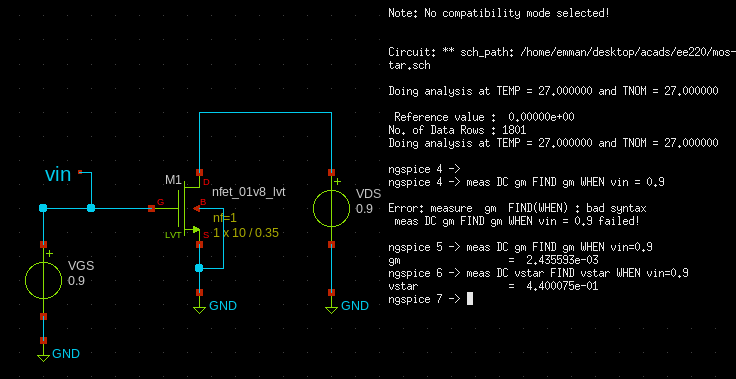
\includegraphics[scale=0.32]{gm-vstar.png}
	\label{label:gm-vstar-NMOS} 
	\caption{$g_m$ and $v^*$}
\end{figure}
The values are obtained by using the MEAS command. Note that the TT corner is used for the simulation. 

\subsection{PMOS Noise}


\end{document}\textsl{}